\expandafter\newcommand\csname dataXGBvifmetrictab\endcsname{
\begin{table}[H]
\begin{tabular}
{| 
 p{\dimexpr0.2\textwidth-2\tabcolsep-\arrayrulewidth\relax}| 
 p{\dimexpr0.2\textwidth-2\tabcolsep-\arrayrulewidth\relax}| 
 p{\dimexpr0.2\textwidth-2\tabcolsep-\arrayrulewidth\relax}| 
 p{\dimexpr0.2\textwidth-2\tabcolsep-\arrayrulewidth\relax}| 
 p{\dimexpr0.2\textwidth-2\tabcolsep-\arrayrulewidth\relax}| 
}\hline 
\textbf{} &\textbf{f1-score} &\textbf{precision} &\textbf{recall} &\textbf{support} \\ \hline 
CANDIDATE &0.637 &0.687 &0.594 &170.0 \\ \hline 
CONFIRMED &0.855 &0.829 &0.884 &241.0 \\ \hline 
FALSE POSITIVE &0.928 &0.92 &0.936 &391.0 \\ \hline 
accuracy &0.848 &0.848 &0.848 &0.848 \\ \hline 
macro avg &0.807 &0.812 &0.805 &802.0 \\ \hline 
weighted avg &0.844 &0.843 &0.848 &802.0 \\ \hline 
\end{tabular} 
\end{table}
}
\begin{figure}[H]
                \centering
                \begin{subfigure}{.49\textwidth}
                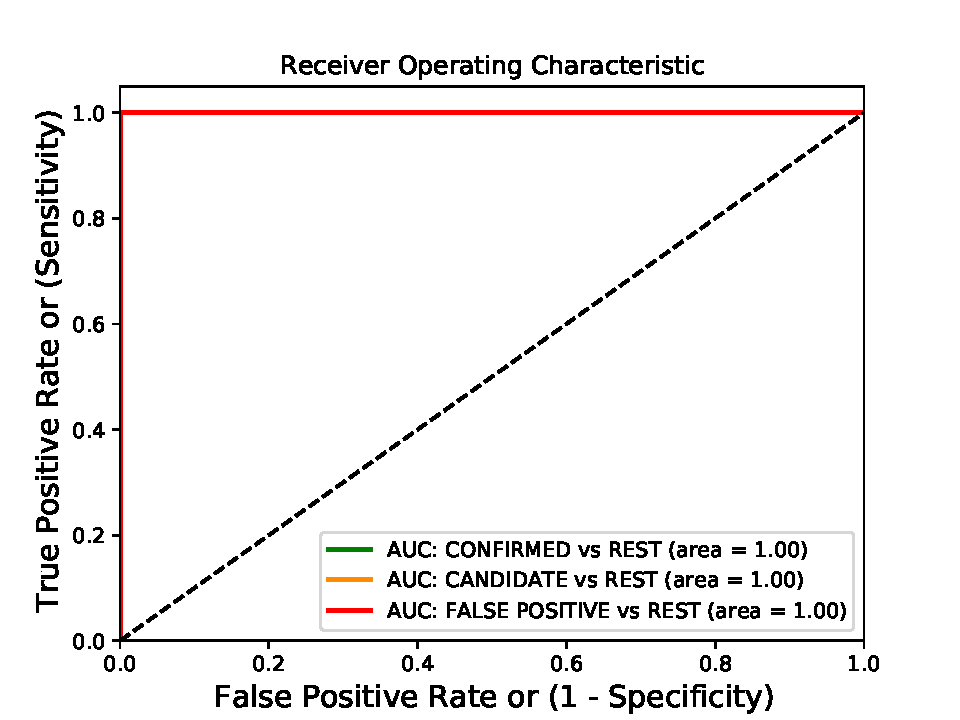
\includegraphics[width = 1\textwidth]{data/XGB_vif_overfit_roc.pdf}
                \end{subfigure}
                \begin{subfigure}{.49\textwidth}
                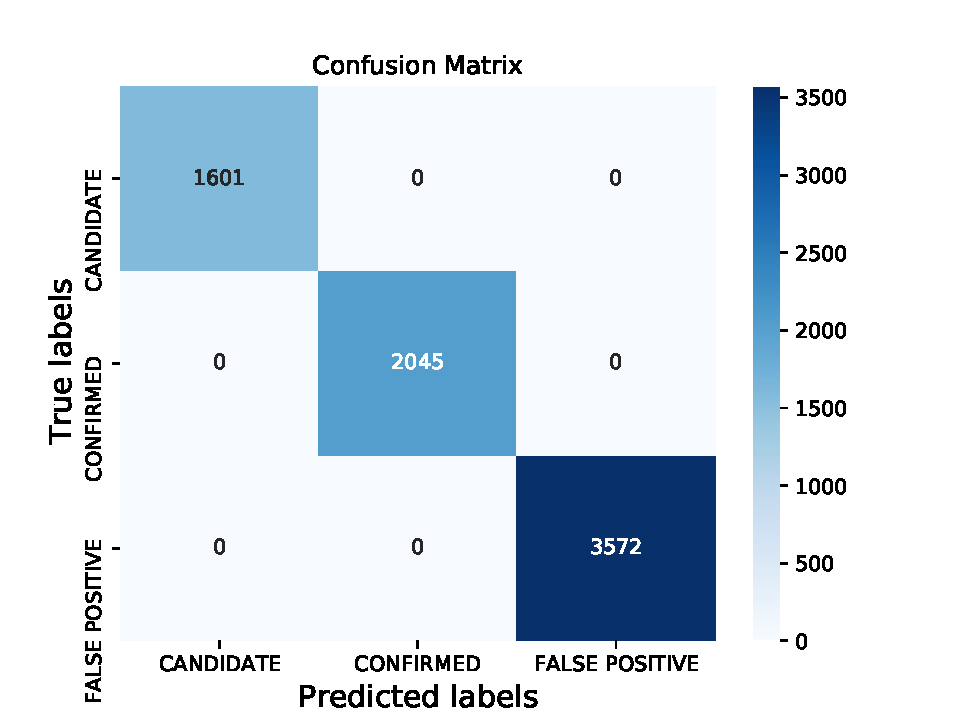
\includegraphics[width = 1\textwidth]{data/XGB_vif_overfit_cm.pdf}
                \end{subfigure}
                \begin{subfigure}{.49\textwidth}
                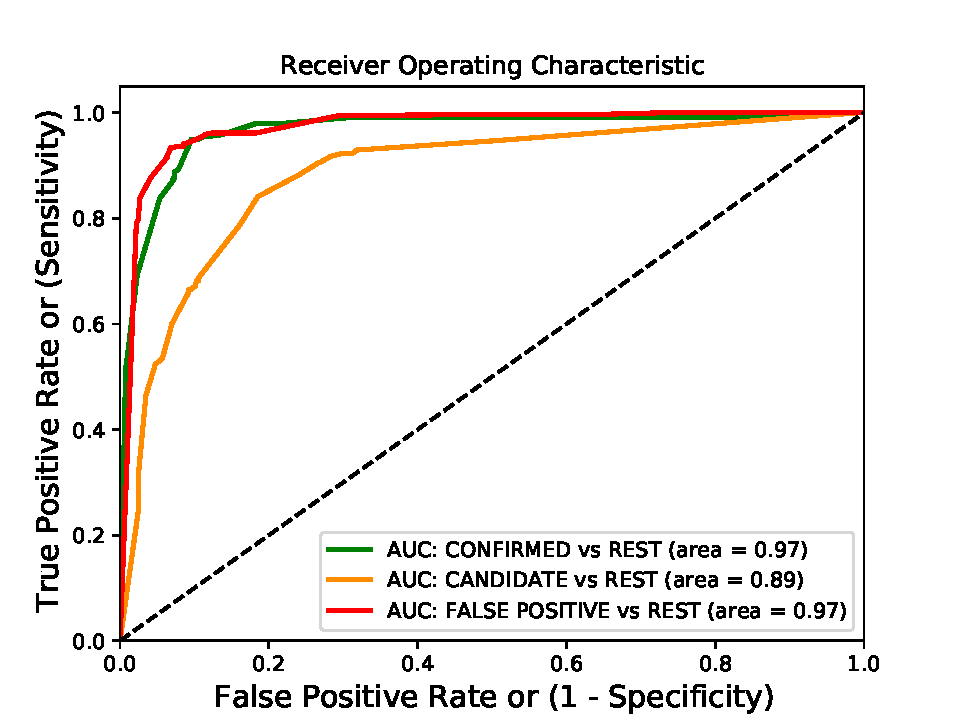
\includegraphics[width = 1\textwidth]{data/XGB_vif_roc.pdf}
                \end{subfigure}
                \begin{subfigure}{.49\textwidth}
                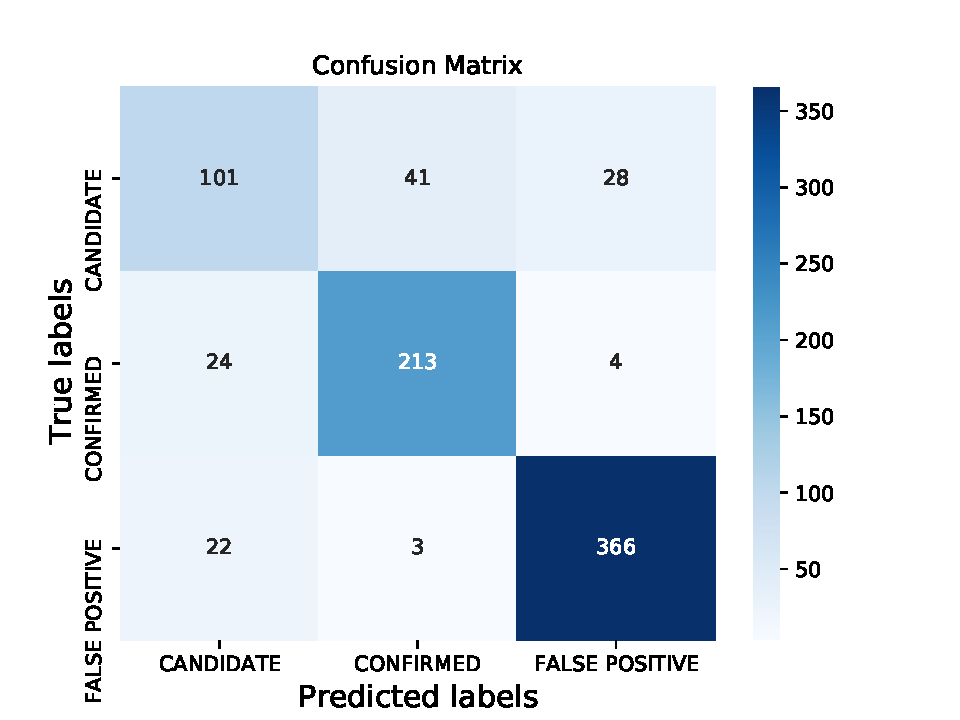
\includegraphics[width = 1\textwidth]{data/XGB_vif_cm.pdf}
                \end{subfigure}
                \begin{subfigure}{1\textwidth}
                \csname dataXGBvifmetrictab\endcsname
                \end{subfigure}
                \caption{XGBvif: Top Row: overfit test. Middle and bottom row test data}
                \label{fig:data/XGB_vif_roc}
                \end{figure}